\documentclass{article}
\usepackage[style=apa, backend=biber]{biblatex}
\addbibresource{hopping.bib}
\usepackage{graphicx}
\usepackage{booktabs}
\usepackage{indentfirst}
\usepackage{amsmath}
\usepackage{setspace}
\usepackage[margin=1in]{geometry}
\usepackage[table,x11names]{xcolor}
\usepackage{fancyhdr}
\usepackage{tabularx}
\usepackage[compact]{titlesec}
\usepackage{listings}
\usepackage{color}
\usepackage{fontspec}
\usepackage{unicode-math}
\pagestyle{fancy}
\fancyhf{}
\renewcommand{\headrulewidth}{0pt}
\fancyhead[R]{\thepage}
\titleformat{\section}[block]{\normalsize\bfseries}{}{0em}{}
\titleformat{\subsection}[block]{\normalsize\bfseries}{}{0em}{\itshape}
\titleformat{\subsubsection}[block]{\normalsize}{}{0em}{\itshape}
\doublespacing
\setmainfont{DejaVu Serif}
\setmathfont{DejaVu Math TeX Gyre}
\setmonofont{DejaVu Sans Mono}
\newfontfamily\listingsfont[Scale=.7]{DejaVu Sans Mono}
\definecolor{dkgreen}{rgb}{0,0.6,0}
\definecolor{gray}{rgb}{0.5,0.5,0.5}
\definecolor{mauve}{rgb}{0.58,0,0.82}

\lstset{frame=tb,
  language=C,
  aboveskip=3mm,
  belowskip=3mm,
  showstringspaces=false,
  columns=flexible,
  basicstyle={\small\ttfamily},
  numbers=none,
  numberstyle=\tiny\color{gray},
  keywordstyle=\color{blue},
  commentstyle=\color{dkgreen},
  stringstyle=\color{mauve},
  breaklines=true,
  breakatwhitespace=true,
  tabsize=3
}

\begin{document}
\begin{titlepage}
	\centering
	\vspace*{0.2\textheight}
	\textbf{Preferred hopping frequency is independent of predictors of cardiorespiratory health}\\
	Lyndsay Ricks\\
	Department of Biology, University of Utah\\
	BIOL 3665: Animal Form and Function\\
	Colleen Farmer\\
	April 14, 2023
\end{titlepage}
\section{Abstract}

{\parindent0pt Hopping is an aerobic exercise with significant biomechanical components. The frequency at which a given person prefers to hop could therefore be influenced by both morphology and cardiorespiratory fitness, yet only the former has been given attention in the literature. Previous research has demonstrated the predictive power with respect to VO$_2$max, a recognized proxy of cardiorespiratory fitness, of several demographic and physiological variables in humans. Here, a set of the same or similar variables are tested for their relationship with preferred hopping frequency in a cohort of college students ($n = 8$), with only height exhibiting significant predictive power. Cardiorespiratory fitness is concluded to be unlikely to be a major contributor to preferred hopping frequency; further research directions are discussed.} \\

{\parindent0pt Keywords: \emph{cardiorespiratory fitness, VO$_2$max, physiology, human biology}}

\pagebreak

\section{Introduction}
The biomechanics of hopping have been the subject of hundreds, if not thousands, of research studies. The subject is of relevance to comparative morphology \parencite{farley1993, lee2014}, physiology \parencite{ferris1997}, and even developmental neurobiology \parencite{beerse2020}, among other fields, and of particular focus in most research on the topic is the mechanics of stiffness and strain in the legs when hopping (see, for example, \cite{ferris1997,mcmahon1990,moholkar2004}). The existence of individually preferred frequencies in hopping tasks has been acknowledged since at least 1971 \parencite{jones1971}, but the fact that these frequencies exist seems to have been taken for granted in much of the literature (for example, in \cite{farley1991}); attempts to search for factors behind them have been at best secondary to different research questions and have yielded rather uninteresting results \parencite{demirbuken2009,granata2002}. However, variation --- consistent, at that, as even \textcite{jones1971} noted --- does exist in preferred frequencies, and the factors behind this variation do warrant investigation.

As hopping is an aerobic exercise, not merely a neutral biomechanical test, one potential factor influencing preferred hopping frequency might be cardiorespiratory fitness. Unfortunately, as ``cardiorespiratory fitness'' is not per se quantifiable, it must be approximated via proxies such as VO$_2$max --- the maximum rate at which oxygen is consumed during physical exertion --- which is the accepted standard metric of cardiorespiratory fitness and has been for decades \parencite{hamlin2014,siconolfi1982}, although it is not without controversy \parencite{green2018}. The process of measuring VO$_2$max is quite intensive and it is typically only feasible within a laboratory setting, however, so various attempts have been made to simplify the process of estimating cardiorespiratory health in situations where measuring VO$_2$max is infeasible due to resource constraints or other concerns \parencite{ashfaq2022,george1996,grant1999}; here, I will be utilizing, with some modifications, the statistical methodology and variables proposed by \textcite{abut2016}, which have the advantage of being numerous, mostly trivial to measure, and drawing from a very similar sample pool to the one available to me. A correlation between predictors of VO$_2$max and preferred hopping frequency would suggest a connection between the latter and cardiorespiratory health, while a lack of a relationship would suggest that preferred hopping frequency may be more related to structural or morphological factors. 

\section{Materials and methods}
\subsection{Participants}
Participants were drawn from a pool of nine undergraduate students enrolled in a biological form and function laboratory course at the University of Utah (Salt Lake City, UT, USA), of whom eight, including the author, ultimately provided all requisite data. Of the participants, five were female and three were male. Apart from age, the demographic and health information provided by participants varied quite widely, as is summarized in Table \ref{fig:summary}, providing a reasonably accurate approximation of the overall population. 
\begin{table}[h!]
\centering
\begin{tabularx}{\linewidth}{Xllll}
\toprule
Variable                                        & Median & Mean  & Standard deviation & Range (min-max) \\ \midrule
Age (years)                                     & 22     & 22.6  & 3.1                & 18-27           \\
Weight (kg)                                     & 66.8   & 70.5  & 13.5               & 58-99           \\
Height (m)                                      & 1.71   & 1.72  & 0.076              & 1.64-1.87       \\
Resting heart rate (bpm)                        & 73.5   & 73.3  & 10.6               & 60-88.5         \\
Heart rate after 20 min moderate exercise (bpm) & 116    & 120.5 & 23.3               & 89-153          \\
Heart rate after 10 min vigorous exercise (bpm) & 135    & 143.5 & 25.0               & 118-182         \\
Sum of answers to PFA questionnaire             & 14.5   & 13.9  & 4.3                & 6-21            \\
Frequency I (calculated via computer)                      & 0.76   & 0.82  & 0.48               & 0.29-1.56       \\
Frequency II (counted manually)                        & 0.73   & 0.80  & 0.44               & 0.33-1.55       \\ \bottomrule
\end{tabularx}
	\caption{Summary statistics for all variables ($n = 8$).}
	\label{fig:summary}
\end{table}

\subsection{Data collection}
Owing to time and budget constraints, not all of the potential predictors of VO$_2$max identified and tested by \textcite{abut2016} could be measured. The various maximal and submaximal metrics they selected were collapsed into a simple measurement of heart rate after 10 minutes of vigorous and 20 minutes of moderate aerobic exercise (selected by the participant). Basic demographic variables were retained, as well as the PFA questionnaire (see Supplementary Material), which was identified as a relatively strong discriminator. The PAR questionnaire was not given to participants, as \textcite{abut2016} found it to be much weaker than the PFA questionnaire. Participants were instructed to obtain their resting heart rate by measuring at four times and calculating the average.

Participants' preferred hopping frequencies were simultaneously measured in two different ways — digitally and manually. For the digital portion, participants utilized Blackboard microcontroller boards and three-dimensional QWIIC accelerometers (both from SparkFun Electronics, Niwot, CO, USA). Participants affixed both the microcontroller board and the attached accelerometer to a chosen stable portion of their body and used the official Arduino IDE (Arduino, Turin, Italy) to execute a script (see Supplementary Material) to obtain acceleration values on all axes at short intervals as they hopped up and down regularly at a pace comfortable to them for a total of 120 seconds. Participants cut the data down to only the middle 60 seconds and identified crests in the resulting waveform (Figure \ref{fig:examplehop} gives an example), reporting the reciprocal of the average distance from each crest to the next along with a standard deviation (Figure \ref{fig:equations}). This value is hereafter referred to as Frequency I. 

\begin{figure}[h!]
\centering
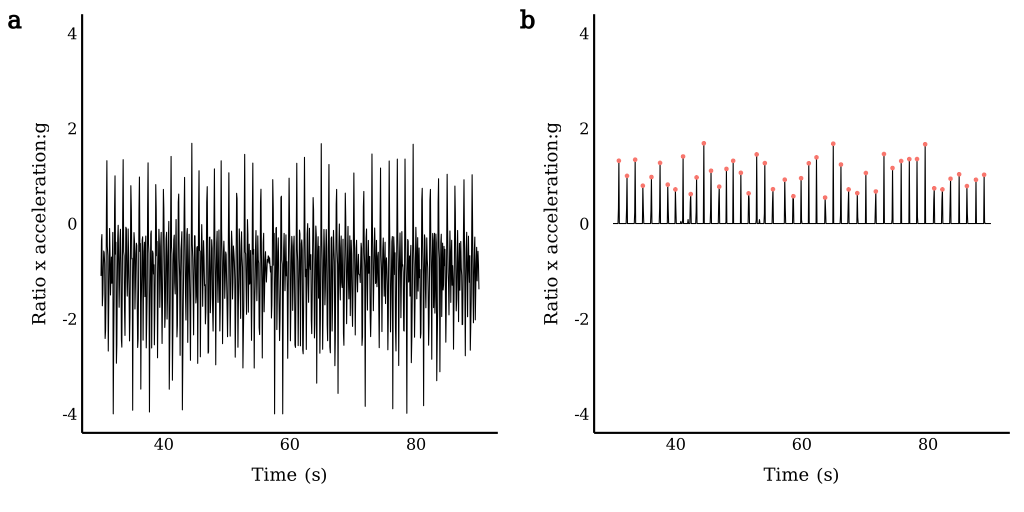
\includegraphics[width=\linewidth]{plots/examplehop.png}
\caption{\centering A real example of hopping data obtained via accelerometer, sampling approximately every 7 ms. (a) Raw data plotted as time vs. acceleration, (b) data reduced to crests only (red dots), which would then be used with the equations in Figure \ref{fig:equations}.}
\label{fig:examplehop}
\end{figure}

\begin{figure}[h!]
\begin{equation}
\bar f = \left(\frac{\sum_{i}^{n} t_i - t_{i - 1}}{n}\right)^{-1}
\end{equation}
\begin{equation}
\sigma_f = \sqrt{\frac{\sum_{i}^{n} ((t_i - t_{i-1})^{-1} - \bar f)}{n}}
\end{equation}
\caption{\centering Equations for calculation of Frequency I, average (1) and standard deviation (2). $t$ indicates the timestamp at which a crest occurs.}
\label{fig:equations}
\end{figure}

In addition to the computerized count, participants manually counted how many times they jumped in the same session and divided this count by the \emph{full} length of time in order to obtain a separate measurement of frequency. This measurement is referred to here as Frequency II. For the most part, Frequencies I and II were very similar, but not identical, within participants' estimates (mean difference $\pm 0.071$ Hz).

\begin{figure}[h!]
	\centering
	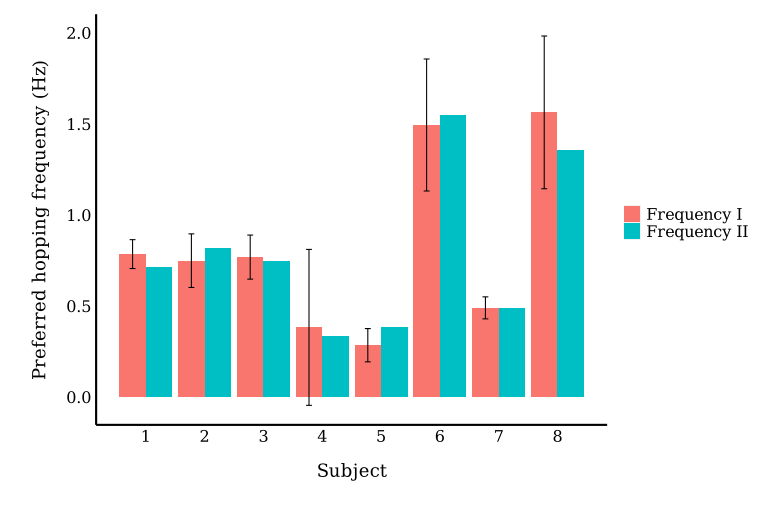
\includegraphics[width=0.75\linewidth]{plots/preference.png}
	\caption{\centering Preferred hopping frequencies among participants (error bars for Frequency I are equal to $\pm\sigma_f$).}
	\label{fig:freqplot}
\end{figure}

All information in the dataset used was self-reported by participants and measured in uncontrolled and potentially unstandardized environments; although participants were given clear general instructions as to how to measure each variable (included in Supplementary Material), the specifics were left to their discretion.

\subsection{Analysis}
Analysis was conducted in R version 4.2.2 \parencite{r} using the packages \texttt{FSinR} \parencite{fsinr} for feature selection; \texttt{data.table} \parencite{datatable}, \texttt{dplyr} \parencite{dplyr}, and \texttt{tidyr} \parencite{tidyr} for data manipulation; and \texttt{ggplot2} \parencite{ggplot2} and \texttt{ggpubr} \parencite{ggpubr} for production of graphics. Relevant features were identified using Relief-F scores at a threshold $F > 0$ (across both frequency counts), determined by visual inspection \parencite{kira1992}. Considering the small sample size and the fact that only three predictors met the Relief-F threshold, it became clear that an SVM-based approach to categorizing the remaining predictors (as was taken by \cite{abut2016}) would be infelicitous. Linear regression analysis was performed instead.

\section{Results}

\begin{table}[h!]
\centering
	\begin{tabularx}{\linewidth}{@{}XllX@{}}
	\toprule
	Predictor                          & Relief-F score (frequency I) & Relief-F score (frequency II) & Outcome                        \\ \midrule
	Age                                & $-0.050295218$                                       & $-0.062225137$                             & Excluded \\
	Sex                                & $0.040612306$                                        & $0.061634546$                              & Retained                       \\
	Weight                             & $0.115953009$                                        & $0.081889255$                              & Retained                       \\
	Height                             & $0.214929358$                                        & $0.254722111$                              & Retained                       \\
	Resting heart rate                 & $-0.064587039$                                       & $-0.067885327$                             & Excluded \\
	Heart rate after moderate exercise & $-0.047876574$                                       & $-0.047648223$                             & Excluded \\
	Heart rate after vigorous exercise & $0.007974116$                                        & $-0.006987602$                             & Excluded \\
	PFA questionnaire                  & $-0.003871271$                                       & $-0.020412946$                             & Excluded \\ 	\bottomrule
	\end{tabularx}
	\caption{Feature selection results.}
	\label{fig:relief}
\end{table}

Only sex, weight, and height exhibited strong enough Relief-F scores to be included in further analysis (Table \ref{fig:relief}). Relief-F scores were mostly similar regardless of which frequency measurement was used as the response variable, but the disparity was generally larger for the three positive predictors. Height exhibited the highest score by far for both frequency measurements.

\begin{table}[h!]
\centering
\begin{tabularx}{\linewidth}{@{}lXlXl@{}}
\toprule
Predictor & $t$ (Frequency I) & $p$ (Frequency I) & $t$ (Frequency II) & $p$ (Frequency II) \\ \midrule
Height    & 2.79                                   & 0.049 **                                 & 2.76                   & 0.051 *                  \\
Weight    & 1.33                                   & 0.25                                     & 0.76                   & 0.49                     \\
Sex       & -0.96                                   & 0.39                                     & -0.76                   & 0.49                     \\ \bottomrule
\end{tabularx}
\caption{\centering Results of linear regression analysis (*marginally significant, $p < 0.1$; **significant, $p < 0.05$).}
\label{fig:lms}
\end{table}

Linear regression using all three selected factors revealed a marginally significant relationship between height and both frequency counts ($p \approx 0.05$), while no significant relationship between hopping frequency and weight or sex (which also had lower Relief-F scores) was apparent (Table \ref{fig:lms}). For Frequency I, the whole-model $p$ was 0.0568 and the $R^2$ was 0.686. For Frequency II, the whole-model $p$ was 0.0790 and the $R^2$ was 0.627.

\begin{table}[h!]
\centering
\begin{tabular}{@{}lll@{}}
\toprule
Response variable & $p$ & $R^2$ \\ \midrule
Frequency I & 0.0151 * & 0.596 \\
Frequency II & 0.00951 ** & 0.6511 \\ \bottomrule
\end{tabular}
\caption{Results of linear regression with height as the sole predictor and either frequency as the response variable  (*significant, $p < 0.05$; **very significant, $p < 0.01$).}
\label{fig:heightlm}
\end{table}

\begin{figure}[h!]
\centering
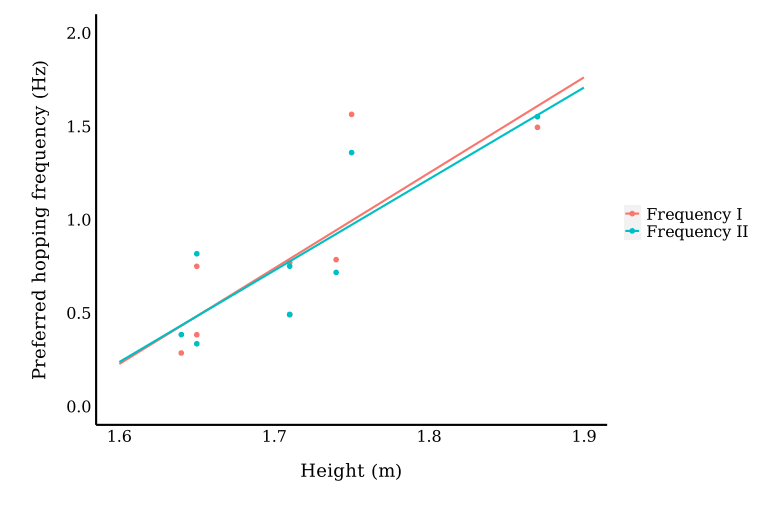
\includegraphics[width=0.75\linewidth]{plots/height.png}
\caption{Hopping frequency as a function of height alone.}
\label{fig:scatter}
\end{figure}

The predictive power of height with respect to hopping frequency when the insignificant extraneous predictors are removed is striking. The $R^2$ of linear regressions conducted with height alone as a predictor is between about 0.6 and 0.65, depending on which frequency measurement is used (Table \ref{fig:heightlm}). Plotting the two frequency measurements against height underscores the relative strength of the linear relationship between the two variables (Figure \ref{fig:scatter}). In the case of Frequency II, a solely height-based model explains slightly more of the variation in preferred hopping frequency than does the original multiple regression model ($R^2$ for height only = 0.651; for multiple predictors = 0.627). Interestingly, in this dataset, there is no correlation between height and weight (presumably a consequence of the small sample size), nor is there a significant interaction effect between the two when predicting either metric of hopping frequency; weight would seem not to be a confounding factor when considering the relationship identified between height and hopping frequency in this dataset.

\section{Discussion and conclusion}

The inherent limitations of this research design temper the extent to which generalizations can be made. First of all, the fact that measurements were performed in an uncontrolled setting adds some amount of uncertainty to the accuracy of the raw data. Weight and height in particular have often been reported throughout the last 40 years of literature to be systematically under- and overestimated when drawn from self-reported data, variously being influenced by other demographic variables such as sex, age, and level of education \parencite{brener2003,engstrom2003,hodge2020,palta1982,spencer2002}, although at least one investigation found accurate self-reporting of these variables in a smaller cohort ($n = 60$) consisting solely of pre-menopausal women \parencite{roth2013}. An examination of these studies indicates that the disparities between self-reported and actual weight/height are typically less than five pounds (usually underestimated) and two inches (usually overestimated, especially among males) respectively, which would be unlikely to be problematic enough to call the validity of the statistics here into question, but does indicate that caution must be exercised when relying on these self-reported variables.

In addition, our inability to measure VO$_2$max for the dataset meant that it was necessary to rely upon previous research establishing predictors thereof without being able to verify that the trends they identified extend to our own cohort --- i.e., it is possible that a composite of the variables used might not even be an adequate proxy of cardiovascular health within this cohort, though there is no way to know for sure. It is worth noting that \textcite{abut2016} recruited college students from Provo, UT, USA, which would be incredibly close demographically to the participants of this study, and it would therefore be surprising for this group to violate the trends \textcite{abut2016} identified, but a more complete investigation of the same question would regardless benefit from directly measuring VO$_2$max.

Finally and perhaps most obviously, this study suffers from the same problem as any other with such a small sample size. Direct points of comparison such that a set of individuals differs only with respect to one variable are essentially nonexistent when considering all of the variables measured, and are still sparse when the variables are narrowed down to only the three selected. This can lead to undesirable noise and also reduce the generalizibility of these results.

The lack of a significant predictive relationship between sex and hopping frequency is unsurprising, as previous research has indicated that although women's leg stiffness differs significantly from males' in stationary hopping tasks, women do not choose different preferred hopping frequencies from males \parencite{demirbuken2009,granata2002}. Likewise, the lack of a clear impact caused by weight is consistent with previous literature; \textcite{gutmann2013} also did not find a relationship between body mass and chosen hopping frequency, although this was not the primary focus of their research.

Despite methodological issues and a lack of predictive power on the part of most of the selected predictors, it remained possible to detect one plausible trend: height positively correlates with preferred hopping frequency. This is an interesting relationship and does not appear to have been explored in the literature previously. It is somewhat unclear how to interpret this relationship, but one possible explanation may be found in the fact that height is likely to be at least broadly a reasonable proxy for leg length; although leg length is also impacted by scaling factors such as nutrition and genetics \parencite{bogin2010}, a generally taller person should also be expected to have generally longer legs (in an absolute sense). If the leg is (reasonably) approximated as a Hookean mass-spring system at its optimal hopping frequency \parencite{blickhan1989}, then for two legs of equal mass, the stiffness constant $k_\textrm{leg} \propto l_0$ \parencite{farley1993,mcmahon1990}. Then, approximating the spring force as $F = k_\textrm{leg}\Delta L$, if the force is the same in either case, $\Delta L \propto (l_0)^{-1}$. In other words, a longer leg would not need to expand and contract as far as a shorter leg in order to produce the same reaction force. The reduction in strain applied to the legs in order to reach the same hopping height could make faster hopping feel physically easier and more preferable for taller individuals, explaining their propensity for higher hopping frequencies. 

This is, of course, a very speculative explanation, and considering the small sample size (and lack of researcher control over the process of measuring height and preferred hopping frequency), it is possible the correlation between preferred hopping frequency and height could even be nothing more tahn an improbably deceptive statistical artifact. The first step in verifying this hypothesis would be to repeat this study on a much larger sample with appropriate researcher oversight and the second would be to use force plate measurements to control for variation in applied forces; it would be inappropriate to make any generalizations before verifying these results in such a manner. 

Irrespective of the role of height, these results indicate that cardiorespiratory fitness is not likely to be a significant factor in observed variability in preferred hopping frequency, although this could be more reliably confirmed in the future by measuring VO$_2$max directly within a larger sample. Despite the large amount of research on the biomechanics of hopping tasks, the factors affecting variation in preferred hopping frequency have been investigated relatively infrequently and typically in a secondary capacity. Considering the paucity of research on the subject and the statistical significance of the trend identified here, the validity of height and more precise metrics of variation in leg biomechanics as predictors of preferred hopping frequency merit further investigation in a larger and more reliable sample. 

\pagebreak
\printbibliography
\pagebreak
\section{Supplementary material}
\subsection{Instructions for data collection}
No specific instructions were given to participants for age, sex, weight, and height other than the units in which to provide them. For the other variables, instructions were as follows.
\subsubsection{Resting heart rate}
For the purposes of this analysis, please do your best to find a relaxing environment and spend at least 10-15 minutes there relaxing (preferably without distractions such as electronics) before taking a pulse. Make a tight fist and locate the pulse point of your radial artery just below your wrist on the thumb side of the large prominent tendon, as depicted below.

\begin{figure}[h!]
\centering
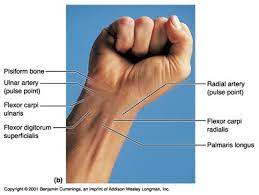
\includegraphics{pics/pulse.jpeg}
\end{figure}

Relax your fist and put pressure with two fingers at the pulse point until you feel a strong and clear pulse. Do NOT use your thumb to take a pulse, as it has its own pulse point and will complicate the results. After feeling 3 consecutive strong pulses, start a timer for 60 seconds or look at a clock for 60 seconds, counting the pulses throughout the whole minute. Record the number of pulses along with the date and time. Do this twice a day (once in the morning and once in the evening) for two consecutive days, recording the numbers each time. 

\begin{figure}[h!]
\centering
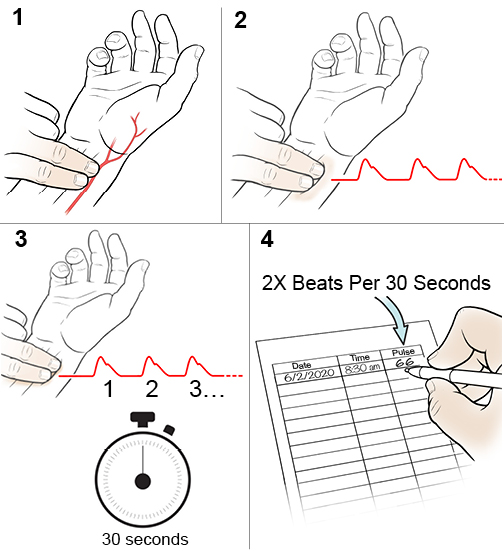
\includegraphics[width=0.6\linewidth]{pics/pulse2.jpeg}
\end{figure}

Average the four measurements you obtained.

\subsubsection{Heart rate with exercise}

Perform 20 minutes of aerobic exercise (jogging, cycling, swimming, etc.) that feels moderate (sustainable for that length of time, but somewhat challenging) and immediately afterwards, measure your heart rate one time the same way you did for your resting heart rate.

Perform 10 minutes of aerobic exercise (jogging, cycling, swimming, etc.) that feels intense/vigorous to you and immediately afterwards, measure your heart rate one time the same way you did for the other two measurements.

\subsubsection{PFA questionnaire}
The questionnaire is embedded below. Select a number between 1 and 13 that fits you for both questions and add the numbers that you chose together. Your result should be between 2 and 26. For example, if I think that jogging between a slow and medium pace is just right for me, and I could jog 3 miles at a pace between fast walking and slow jogging, I would answer 8+6 = 14.

\begin{figure}[h!]
\centering
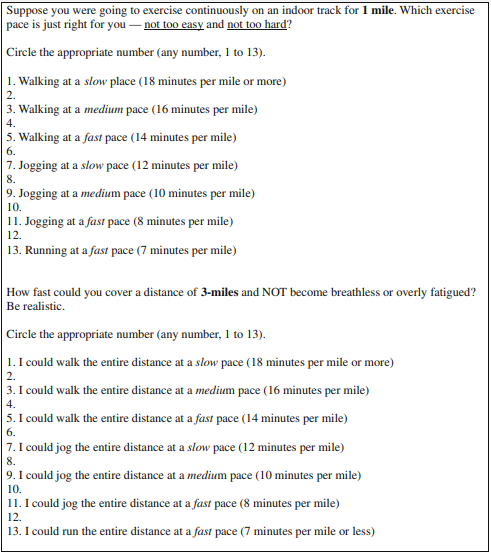
\includegraphics[width=0.8\linewidth]{pics/pfa.png}
\caption{PFA questionnaire provided to participants \parencite{akay2009}.}
\end{figure}

\pagebreak
\subsection{Raw data and scripts}

\subsubsection{Arduino script}

The following script was used by participants to obtain their acceleration (provided by Mark Howell):
\begin{lstlisting}[basicstyle=\linespread{0.3}\listingsfont]
#include <Wire.h>                 // Must include Wire library for I2C
#include "SparkFun_MMA8452Q.h"    // Click here to get the library: http://librarymanager/All#SparkFun_MMA8452Q
#include <math.h>

MMA8452Q accel;                   // create instance of the MMA8452 class

// Declare and initialize variables for acceleration readings
float xAccel = 0.;
float yAccel = 0.;
float zAccel = 0.;
float accelMag = 0.;
float correctionFactor = 2.0; // Needed for scales other than 2G, use 2 for 4G and 4 for 8G
long currentTime = 0L;
long checkTime = 0L;
int delayTime = 0;


// Sample rate, in Hz
float sampleRate = [selected by participant; >10];

void setup() {
    Serial.begin(115200);
    Wire.begin();
    if (accel.begin() == false) {
        Serial.println("Not Connected. Please check connections and read the hookup guide.");
        while (1);
    }
    //Adjust sensitivity to +- 4G, should prevent saturation
    accel.setScale(SCALE_4G);
    delayTime = 1000/sampleRate;
}

void loop() {
    while (Serial.available() == 0) 
    {
        if (accel.available()) {      // Wait for new data from accelerometer
            currentTime = millis();
            // Acceleration of x, y, and z directions in g units
            xAccel = accel.getCalculatedX() * correctionFactor;
            yAccel = accel.getCalculatedY() * correctionFactor;
            zAccel = accel.getCalculatedZ() * correctionFactor; 
            // Determine magnitude of acceleration vector
            // Determine magnitude of acceleration vector
            accelMag = sqrt(xAccel*xAccel + yAccel*yAccel + zAccel*zAccel);
            //checkTime = currentTime + delayTime;
            Serial.print("x = ");
            Serial.print("\t");
            Serial.print(xAccel, 3);
            Serial.print("\t");
            Serial.print("y = ");
            Serial.print("\t");
            Serial.print(yAccel, 3);
            Serial.print("\t");
            Serial.print("z = ");
            Serial.print("\t");
            Serial.print(zAccel, 3);
            Serial.print("\t");
            Serial.print("Mag = ");
            Serial.print("\t");
            Serial.print(accelMag, 3);
            Serial.print("\t");
            Serial.print("time = ");
            Serial.print("\t");
            Serial.print(currentTime/1000.,3);
            Serial.println();
            while (millis() < (currentTime + delayTime))
            {
                // Wait until enough time has passed for the next sensor check
            }
        }
    }
}
\end{lstlisting}

\subsubsection{Statistical analysis and raw data}
The R script for all analyses conducted for this project, the raw data, and the source code for this document are accessible via GitHub at https://www.github.com/lyndsayricks/biol3665.
\end{document}
